\documentclass{article}

\usepackage{graphicx}
\usepackage{tikz}
\usepackage{tikzsymbols}
\usetikzlibrary{calc,patterns,shapes.geometric}
\pagestyle{empty}
\usepackage[margin=0pt]{geometry}
\geometry{papersize={14in,12in}}

\def\centerarc[#1](#2)(#3:#4:#5){\draw[#1] ($(#2)+({#5*cos(#3)},{#5*sin(#3)})$) arc (#3:#4:#5);}

\begin{document}
	\begin{figure}
		\centering
		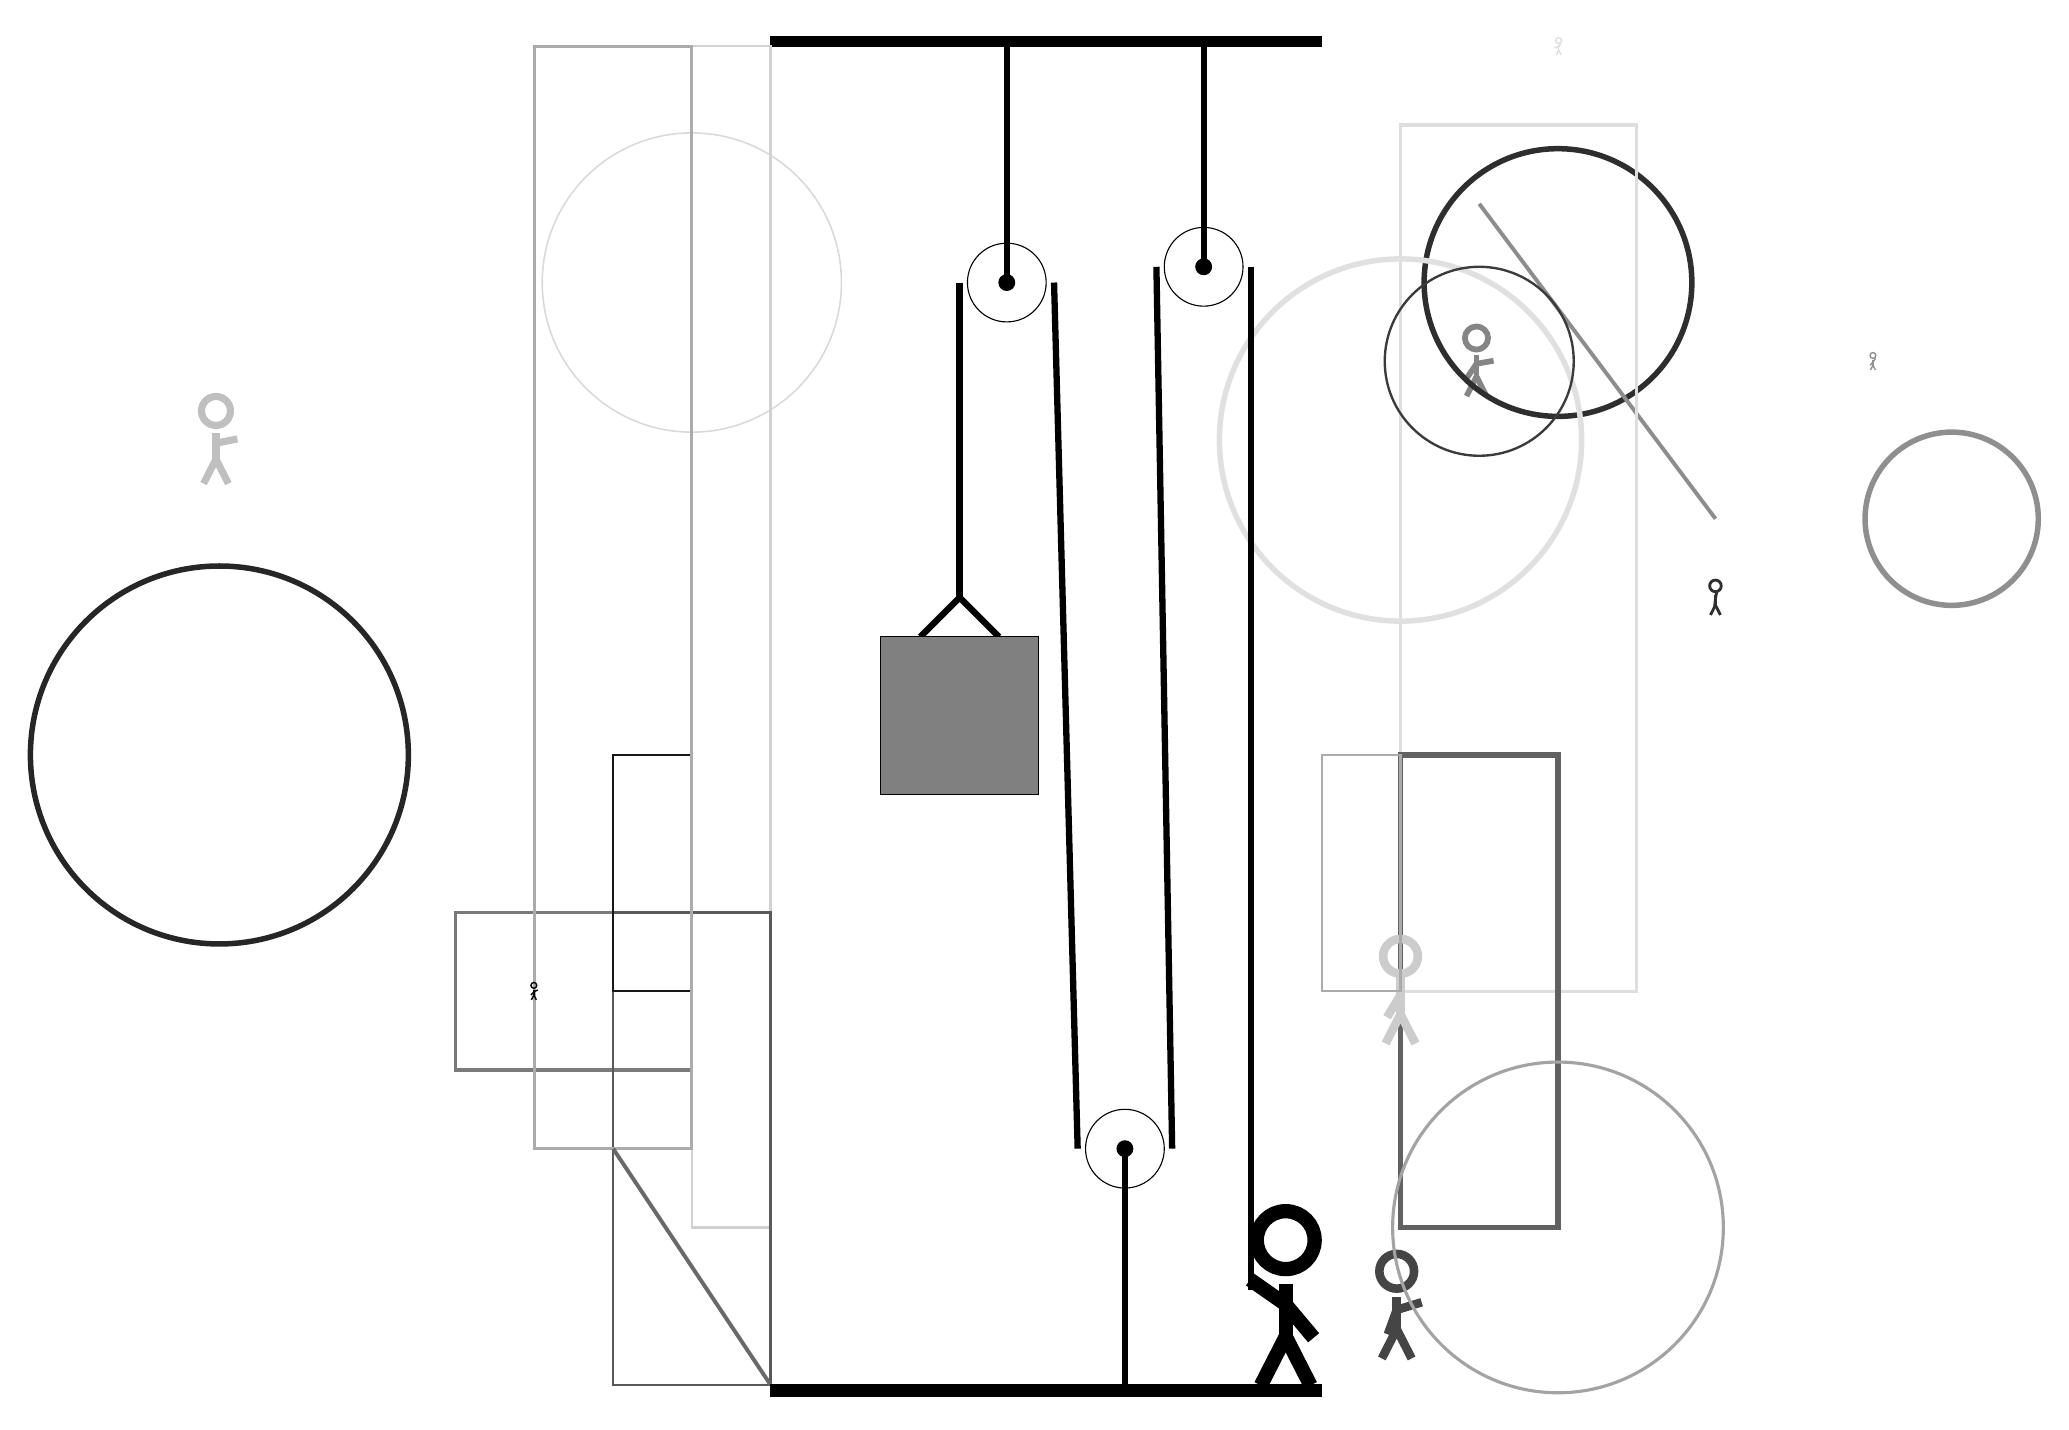
\begin{tikzpicture}
			%%%%% START %%%%%
			
			\draw[fill=black] (-2, 14) rectangle (5, 14.125);
			
			\draw (1, 11) circle (0.5);
			\draw[fill=black] (1, 11) circle (0.1);
			\draw[line width=0.8mm]  (1, 14) -- (1, 11);
			
			\draw[fill=white](2.5, 0) circle (0.5);
			\draw[fill=black] (2.5, 0) circle (0.1);
			\draw[line width=0.8mm]  (2.5, -3) -- (2.5, 0);
			
			\draw[fill=white](3.5, 11.2) circle (0.5);
			\draw[fill=black] (3.5, 11.2) circle (0.1);
			\draw[line width=0.8mm] (3.5, 14) -- (3.5, 11.2);
			
			\node[line width=0.6mm, color=black!48] at (7, 10) {\Strichmaxerl[4][56][10]};
			
			\draw [line width=0.7mm, color=black!82](8, 11) circle (1.7);
			\draw [line width=0.2mm, color=black!15](-3, 11) circle (1.9);
			\draw[line width=0.5mm, color=black!45](10, 8) -- (7, 12);
			
			\draw[line width=0.4mm, color=black!13] (6, 13) rectangle (9, 2);
			
			\draw[line width=0.3mm, color=black!18] (-2, -1) rectangle (-3, 14);
			
			\node[line width=0.3mm, color=black!25] at (-9, 9) {\Strichmaxerl[5][89][11]};
			\draw[line width=0.7mm, color=black!62] (6, -1) rectangle (8, 5);
			\draw[line width=0.4mm, color=black!52] (-3, 3) rectangle (-6, 1);
			
			\draw[line width=0.3mm, color=black!65] (-2, -3) rectangle (-4, 3);
			
			\draw[line width=0.2mm, color=black!91] (-3, 5) rectangle (-4, 2);
			\node[line width=0.6mm, color=black!81] at (10, 7) {\Strichmaxerl[2][84][80]};
			\node[line width=0.4mm, color=black!73] at (6, -2) {\Strichmaxerl[6][70][17]};
			
			\draw [line width=0.7mm, color=black!12](6, 9) circle (2.3);
			\draw [line width=0.3mm, color=black!77](7, 10) circle (1.2);
			\draw[line width=0.4mm, color=black!33] (-3, 14) rectangle (-5, 0);
			
			\draw [line width=0.7mm, color=black!85](-9, 5) circle (2.4);
			\node[line width=0.4mm, color=black!20] at (6, 2) {\Strichmaxerl[6][59][90]};
			\draw[line width=0.3mm, color=black!33] (6, 2) rectangle (5, 5);
			\node[line width=0.7mm, color=black!97] at (-5, 2) {\Strichmaxerl[1][48][25]};
			\draw [line width=0.7mm, color=black!44](13, 8) circle (1.1);
			
			\draw[line width=0.5mm, color=black!59](-4, 0) -- (-2, -3);
			\node[line width=0.6mm, color=black!13] at (8, 14) {\Strichmaxerl[1][12][60]};
			\node[line width=0.7mm, color=black!43] at (12, 10) {\Strichmaxerl[1][51][52]};
			\draw [line width=0.4mm, color=black!36](8, -1) circle (2.1);
			
			
			\draw[line width=0.8mm] (-0.1, 6.5) -- (0.4, 7.0) -- (0.9, 6.5);
			\draw[fill=black!50] (-0.6, 6.5) rectangle (1.4, 4.5);
			
			\draw[line width=0.8mm] (0.4, 11) -- (0.4, 7.0);
			\centerarc[line width=0.8mm](1, 11)(0:180:0.6);
			\draw[line width=0.8mm](1.6, 11) -- (1.9, 0);
			\centerarc[line width=0.8mm](2.5, 0)(180:360:0.6);
			\draw[line width=0.8mm](3.1, 0) -- (2.9, 11.2);
			\centerarc[line width=0.8mm](3.5, 11.2)(0:180:0.6);
			\draw[line width=0.8mm](4.1, 11.2) -- (4.1, -1.8);
			
			\node at (4.5, -1.9) {\Strichmaxerl[10][-35][-50]};
			
			\draw[fill=black] (-2, -3) rectangle (5, -3.15);
			
			%%%%% END %%%%%
		\end{tikzpicture}
	\end{figure}	
\end{document}